\documentclass[11pt,a4paper]{article}
\usepackage[utf8]{inputenc}
\usepackage[spanish,es-tabla]{babel}
\usepackage{amsmath}
\usepackage{amsfonts}
\usepackage{amssymb}
\usepackage{graphicx}
\usepackage{natbib}
\usepackage{lineno}
\usepackage{ragged2e}
\usepackage{multicol}
\setlength\columnsep{38pt}
\usepackage{enumerate} 
\usepackage[left=2.8cm,top=2.3cm,right=2.8cm,bottom=2.3cm]{geometry} 
\usepackage{fancyhdr}
\usepackage{url}
\usepackage{float}

\begin{document}
	
	\begin{center}
		\huge \textbf{Data Warehouse VS. Data Lake} 
	\end{center}
	\vspace{\baselineskip}
	\begin{center}
		
\includegraphics[scale=0.37]{./Imagenes/logo}
	\end{center}
	\vspace{\baselineskip}
	\begin{multicols}{2}
		\small
		\begin{center}
			Nelia Escalante Marón\\
			2014049551\\
			UPT – Ingeniería de Sistemas\\
			EPIS\\
			Tacna, Perú\\
			\vspace{\baselineskip}
			Yerson Coaquira Calizaya\\
			2015053225\\
			UPT – Ingeniería de Sistemas\\  
			EPIS\\
			Tacna, Perú\\                 
			\vspace{\baselineskip}
			Flor Condori Gutierrez\\
			2015053227\\
			UPT – Ingeniería de Sistemas\\  
			EPIS\\	
			Tacna, Perú\\                 
			\columnbreak
			
			\vspace{\baselineskip}
			Christian Cespedes Medina\\
			2010036256\\
			UPT – Ingeniería de Sistemas\\  
			EPIS\\	
			Tacna, Perú\\                 
			
			\vspace{\baselineskip}
			Javier Octavio Arteaga Ramos \\
			2007028981\\
			UPT – Ingeniería de Sistemas\\  
			EPIS\\	
			Tacna, Perú\\                 
			
		\end{center}
		\normalsize			
	\end{multicols}
	\vspace{\baselineskip}
	
	\textbf{\textit{\large Resumen}}\rule[1.5mm]{5mm}{0.1mm}		
	Un lago de datos es diferente, porque almacena datos relacionales de aplicaciones de línea de negocios y datos no relacionales de aplicaciones móviles, dispositivos IoT y redes sociales. La estructura de los datos o el esquema no se define cuando se capturan los datos. Esto significa que puede almacenar todos sus datos sin un diseño cuidadoso o la necesidad de saber para qué preguntas podría necesitar respuestas en el futuro.

Seguramente han escuchado muchas veces el término de Data Warehouse; podemos definirla como una base de datos corporativa donde se integra y depura información de una o varias fuentes distintas, que luego serán procesadas y analizadas desde distintos puntos de vista con afinidad de perspectivas y grandes velocidades de respuesta.

	\rule{155mm}{0.1mm}	

	%\newpage
	\vspace{\baselineskip}

	\textbf{\textit{\large Abstract}}\rule[1.5mm]{5mm}{0.1mm} 		
	\textit{
		A lake of data is different, because it stores relational data from business line applications and non-relational data from mobile applications, IoT devices and social networks. The structure of the data or the schema is not defined when the data is captured. This means that you can store all your data without careful design or the need to know for which questions you might need answers in the future. 
Surely you have heard the term Data Warehouse many times; we can define it as a corporate database where information is integrated and filtered from one or several different sources, which will then be processed and analyzed from different points of view with affinity of perspectives and great response speeds.
	}
			
	%\rule{155mm}{0.1mm}
	
	\vspace{\baselineskip}
	
	\section{Introducción}
	
	Dependiendo de los requisitos, una organización típica requerirá tanto un almacén de datos como un lago de datos, ya que responden a diferentes necesidades y casos de uso.\\
		\\
		Un almacén de datos es una base de datos optimizada para analizar datos relacionales provenientes de sistemas transaccionales y aplicaciones de línea de negocios. La estructura de datos y el esquema se definen de antemano para optimizar las consultas SQL rápidas, donde los resultados se utilizan normalmente para informes y análisis operativos. Los datos se limpian, enriquecen y transforman para que puedan actuar como la "fuente única de verdad" en la que los usuarios pueden confiar.\\
		\\
		 Se pueden usar diferentes tipos de análisis en sus datos, como consultas SQL, análisis de big data, búsqueda de texto completo, análisis en tiempo real y aprendizaje automático para descubrir información.\\
		\\
		A medida que las organizaciones con almacenes de datos ven los beneficios de los lagos de datos, están evolucionando para que incluyan lagos de datos y habiliten diversas capacidades de consulta, casos de uso de la ciencia de datos y capacidades avanzadas para descubrir nuevos modelos de información. Gartner denomina a esta evolución como "Solución de gestión de datos para análisis" o "DMSA".
	
	\section{Marco Teórico}
	
		\subsection{Data Lake}
		
		Un data lake es un repositorio de almacenamiento que contienen una gran cantidad de datos en bruto y que se mantienen allí hasta que sea necesario. A diferencia de un data warehouse jerárquico que almacena datos en ficheros o carpetas, un data lake utiliza una arquitectura plana para almacenar los datos.\\
		\\
		Un data lake es un repositorio centralizado que le permite almacenar todos sus datos estructurados y no estructurados a cualquier escala. Puede almacenar sus datos como están, sin tener que estructurar primero los datos y ejecutar diferentes tipos de análisis, desde cuadros de mandos y visualizaciones hasta procesamiento de big data, análisis en tiempo real y aprendizaje automático para guiar mejores decisiones.
		
		\begin{figure}[H]
			\begin{center}
				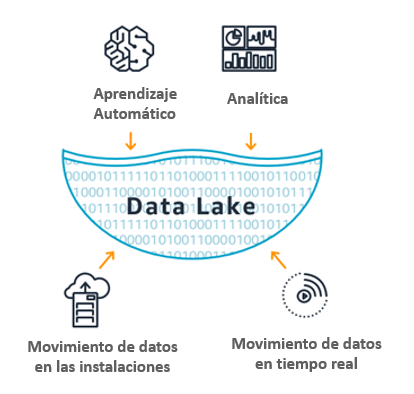
\includegraphics[scale=0.6]{./Imagenes/img01}	
				\caption{Componentes del DataLake}		
			\end{center}
		\end{figure}
	
		A cada elemento de una data lake se le asigna un identificador único y se etiqueta con un conjunto de etiquetas de metadatos extendidas. Cuando se presenta una cuestión de negocios que debe ser resuelta, podemos solicitarle al data lake los datos que estén relacionados con esa cuestión. Una vez obtenidos podemos analizar ese conjunto de datos más pequeño para ayudar a obtener una respuesta.\\
		\\
		El data lake se asocia a menudo con el almacenamiento de objetos orientado a Hadoop. En este escenario, los datos de una organización se cargan primero en la plataforma Hadoop y, a continuación, se aplican las herramientas de análisis y de minería de datos a los datos que residen en los nodos clúster de Hadoop.\\
		\\
		Al igual que con big data, el término data lake a veces se desacredita diciendo que es una simple etiqueta de marketing para un producto que soporta Hadoop. Cada vez más, sin embargo, el término está siendo aceptado como una forma de describir cualquier gran conjunto de datos en el que el esquema y los requisitos de datos no se definen hasta que los datos se consultan.\cite{DLake01:Online}
		
			\subsubsection{Beneficios de una Data Lake}
			
			El principal beneficio de un data lake es la centralización de fuentes de contenido dispares. Una vez reunidas (de sus "silos de información"), estas fuentes pueden ser combinadas y procesadas utilizando big data, búsquedas y análisis que de otro modo hubieran sido imposibles. Las fuentes de contenido dispares a menudo contienen información confidencial que requerirá la implementación de las medidas de seguridad apropiadas en el data lake.\\
			\\
			Las medidas de seguridad en el data lake pueden ser asignadas de manera que se otorga acceso a cierta información a los usuarios del data lake que no tienen acceso a la fuente de contenido original. Estos usuarios tienen derecho a la información, pero no pueden acceder a ella en su fuente por alguna razón.\\
			\\
			Es posible que algunos usuarios no necesiten trabajar con los datos en el origen de contenido original, sino consumir los datos resultantes de los procesos incorporados a dichos orígenes. Puede haber un límite de licencias para el origen de contenido original que impide que algunos usuarios obtengan sus propias credenciales. En algunos casos, la fuente de contenido original se ha bloqueado, está obsoleta o se desactivará en breve, sin embargo, su contenido sigue siendo valioso para los usuarios del data lake.\\
			\\
			Una vez que el contenido está en el data lake, puede normalizarse y enriquecerse. Esto puede incluir extracción de metadatos, conversión de formatos, aumento, extracción de entidades, reticulación, agregación, des-normalización o indexación.\\
			\\
			Los datos se preparan "según sea necesario", lo que reduce los costos de preparación sobre el procesamiento inicial (tal como sería requerido por los data warehouses. Una estructura de big data permite escalar este procesamiento para incluir los conjuntos de datos más grandes posibles.\\
			\\
			Los usuarios, de diferentes departamentos, potencialmente dispersos por todo el mundo, pueden tener acceso flexible a un data lake y a su contenido desde cualquier lugar. Esto aumenta la reutilización del contenido y ayuda a la organización a recopilar más fácilmente los datos necesarios para impulsar las decisiones empresariales.\\
			\\
			La información es poder, y un data lake pone la información de toda la empresa en manos de muchos más empleados para hacer a la organización un todo más inteligente, más ágil y más innovadora.

			\subsubsection{Caracteristicas del Data Lake}
			
				A continuación, destacaremos cinco elementos diferenciadores clave de un data lake y cómo contrastan con el enfoque del data warehouse.
			
			\begin{enumerate}[A.]
				\item \textbf{Una Data Lake conserva todos los datos}
				
				Durante el desarrollo de un data warehouse, se gasta una cantidad considerable de tiempo analizando las fuentes de datos, entendiendo los procesos de negocio y perfilando los datos. El resultado es un modelo de datos altamente estructurado diseñado para la generación de informes. Una gran parte de este proceso incluye tomar decisiones sobre qué datos incluir y no incluir en el almacén. Generalmente, si los datos no se utilizan para responder a preguntas específicas o en un informe definido, pueden excluirse del almacén. Esto se hace generalmente para simplificar el modelo de datos y también para conservar el costoso espacio en el almacenamiento de disco que se utiliza para hacer el data warehouse.\\
				\\
				En contraste, el data lake conserva todos los datos. No sólo los datos que se utilizan actualmente, sino los datos que se pueden utilizar e incluso los datos que nunca se van a ser utilizados sólo porque quizás podrían ser utilizados algún día. Los datos también se mantienen todo el tiempo para que podamos volver en el tiempo a cualquier punto para hacer el análisis.\\
				\\
				Este enfoque se hace posible porque el hardware para un data lake suele ser muy diferente del utilizado para un data warehouse. La ampliación de un data lake a terabytes y petabytes puede hacerse de manera bastante económica.
				
				\item \textbf{Un Data Lake soporta todos los tipos de datos}
				
				Los data warehouses generalmente se componen de datos extraídos de sistemas transaccionales junto con métricas cuantitativas y los atributos que las describen. Las fuentes de datos no tradicionales, como los registros del servidor web, los datos de sensores, la actividad de las redes sociales, el texto y las imágenes, se ignoran en gran medida. Se siguen encontrando nuevos usos para estos tipos de datos, pero consumirlos y almacenarlos puede ser costoso y difícil.\\
				\\
				El enfoque del data lake abarca estos tipos de datos no tradicionales. En el data lake, guardamos todos los datos independientemente de la fuente y la estructura. Los mantenemos en su forma bruta y sólo los transformamos cuando estamos listos para usarlos. Este enfoque se conoce como "Schema on Read" en comparación con el "Schema on Write" que es el enfoque utilizado en el data warehouse
				
				\item \textbf{Un Data Lakes soporta a todos los usuarios}
				
				En la mayoría de las organizaciones, el 80\% o más de los usuarios son "operacionales". Quieren obtener sus informes, ver sus KPIs o seleccionar el mismo conjunto de datos en una hoja de cálculo todos los días. El data warehouse suele ser ideal para estos usuarios porque está bien estructurado, fácil de usar y comprender y está diseñado para responder a sus preguntas.\\
				\\
				El siguiente 10\% más o menos, hace más análisis en esos datos. Utilizan el data warehouse como una fuente, pero a menudo vuelven a los sistemas de origen para obtener datos que no están incluidos en el almacén y a veces traen datos de fuera de la organización. Su herramienta favorita es la hoja de cálculo y crean nuevos informes que a menudo se distribuyen en toda la organización. El data warehouse es su fuente de acceso a los datos, pero a menudo van más allá de sus límites.\\
				\\
				Por último, el restante tanto por ciento de los usuarios hace un análisis profundo. Pueden crear fuentes de datos totalmente nuevas basadas en la investigación. Ellos mezclan muchos tipos diferentes de datos y llegan a nuevas preguntas que deben responderse. Estos usuarios pueden utilizar el data warehouse, pero a menudo lo ignoran, ya que normalmente se les solicita que vayan más allá de sus capacidades. Estos usuarios incluyen a los científicos de datos y pueden utilizar avanzadas herramientas analíticas y capacidades como el análisis estadístico y el modelado predictivo.\\
				\\
				El enfoque del data lake soporta igualmente a todos estos usuarios. Los científicos de datos pueden ir al data lake y trabajar con el gran y variado conjunto de datos que necesitan, mientras que otros usuarios hacen uso de vistas más estructuradas de los datos proporcionadas para su uso.
				
				\item \textbf{Los Data Lakes se adaptan fácilmente a los cambios}
				
				Una de las principales quejas sobre los data warehouses es cuánto tiempo se tarda en cambiarlos. Un tiempo considerable se gasta por adelantado durante el desarrollo de la estructura del almacén. Un buen diseño de almacén puede adaptarse al cambio, pero debido a la complejidad del proceso de carga de datos y al trabajo realizado para facilitar el análisis y la elaboración de informes, estos cambios necesariamente consumirán algunos recursos de desarrolladores y tomarán algún tiempo.\\
				\\
				Muchas preguntas comerciales no pueden esperar a que el equipo del data warehouse adapte su sistema para responderlas. La necesidad cada vez mayor de respuestas más rápidas es lo que ha dado lugar al concepto de auto-servicio de inteligencia empresarial.\\
				\\
				En el data lake, por otro lado, como todos los datos se almacenan en bruto y siempre con accesibles a alguien que necesite utilizarlos, los usuarios tienen el poder de ir más allá de la estructura del almacén para explorar datos de nuevas maneras y responder a sus preguntas a su ritmo.\\
				\\
				Si se demuestra que el resultado de una exploración es útil y existe el deseo de repetirlo, entonces se puede aplicar un esquema más formal y se puede desarrollar la automatización y la reutilización para ayudar a extender los resultados a un público más amplio. Si se determina que el resultado no es útil, puede descartarse y no se han realizado cambios en las estructuras de datos ni se han consumido recursos de desarrollo.\\
				\\
				Descárgate aquí la guía "Data Lake: Superando las limitaciones del Data Warehouse" y descubre todo lo que necesitas saber. 
				
				\item \textbf{Los Data Lakes proporcionan una visión más rápida}
				
				Esta última diferencia es realmente el resultado de las otras cuatro. Debido a que los data lakes contienen todos los datos y tipos de datos, y a que permite a los usuarios acceder a los datos antes de que se hayan transformado, limpiado y estructurado, permite a los usuarios llegar a sus resultados más rápido que el método tradicional de data warehouse.\\
				\\
				Sin embargo, este acceso temprano a los datos tiene un precio. El trabajo típicamente realizado por el equipo de desarrollo de data warehouse no se puede hacer para algunas o todas las fuentes de datos requeridas para realizar un análisis. Esto permite a los usuarios explorar y usar los datos como mejor les parezca, pero el primer nivel de usuarios de negocios que he descrito anteriormente tal vez no quiera hacer ese trabajo. Todavía quieren sus informes y KPI's.\\
				\\
				En los data lakes, estos consumidores de informes operativos harán uso de vistas más estructuradas de los datos en el data lake que se parecen a lo que siempre han tenido antes en el data warehouse. La diferencia es que estas vistas existen principalmente como metadatos que se sitúan sobre los datos en el lago en lugar de tablas físicamente rígidas que requieren un desarrollador para cambiarlas. \cite{DLake02:Online}
				
				
			\end{enumerate}
			
			
			\subsection{Data Warehouse}
			
			El término Datawarehouse fue acuñado por primera vez por Bill Inmon, y se traduce literalmente como almacén de datos, lo definió como una colección de datos orientada a temas concretos, no volátil, integrada y variante en el tiempo, que ayuda a la dirección de una empresa u organización, en la toma de decisiones.\\
			\\
			Pese a las similitudes logísticas que puedan derivarse de la nomenclatura, quienes saben qué es un data warehouse tienen claro que se trata de mucho más que un simple almacén de datos. Aunque podría definirse como un espacio de almacenamiento permanente de información, hay que puntualizar que en él se recogen los datos necesarios para apoyar la presentación de informes, el análisis y otras funciones de BI.\\
			\\
			El estadio previo para plantearse qué es un data warehouse y empezar a trabajar con uno en la organización suele definirse por datos guardados en diferentes lugares, tantos como sistemas de origen. El problema de este enfoque es la falta de integración, algo que resuelve el almacén de datos.\\
			\\
			Para algunos casos, la utilización del repositorio de datos, por ejemplo, en empresas bancarias, ayuda a determinar fraudes en tarjetas de crédito o débito; en telecomunicaciones, proyecta el comportamiento de clientes para brindarle programas de incentivos para que permanezcan en la organización.\cite{DWarehouse01:Online}
			
			\subsubsection{Estructura de un Data Warehouse}
			
			La arquitectura de un data warehouse puede ser dividida en tres estructuras simplificadas: básica, básica con un área de ensayo y básica con área de ensayo y data marts.
			
			\begin{itemize}
				\item \textbf{Con una estructura básica}, sistemas operativos y archivos planos proporcionan datos en bruto que se almacenan junto con metadatos. Los usuarios finales pueden acceder a ellos para su análisis, generación de informes y minería.
								
		        \item \textbf{Al añadir un área de ensayo} que se puede colocar entre las fuentes de datos y el almacén, ésta proporciona un lugar donde los datos se pueden limpiar antes de entrar en el almacén. Es posible personalizar la arquitectura del almacén para diferentes grupos dentro de la organización.
		        
		        \item \textbf{Se puede hacer agregando data marts}, que son sistemas diseñados para una línea de negocio en particular. Se pueden tener data marts separados para ventas, inventario y compras, por ejemplo, y los usuarios finales pueden acceder a datos de uno o de todos los data marts del departamento.
				
			\end{itemize}
			
			\subsubsection{Características de un Data Warehouse}
			
				\begin{itemize}
					\item \textbf{Integrado}: los datos almacenados en el datawarehouse deben integrarse en una estructura consistente, por lo que las inconsistencias existentes entre los diversos sistemas operacionales deben ser eliminadas. La información suele estructurarse también en distintos niveles de detalle para adecuarse a las distintas necesidades de los usuarios.
					
					\item \textbf{Temático}: sólo los datos necesarios para el proceso de generación del conocimiento del negocio se integran desde el entorno operacional. Los datos se organizan por temas para facilitar su acceso y entendimiento por parte de los usuarios finales. Por ejemplo, todos los datos sobre clientes pueden ser consolidados en una única tabla del datawarehouse. De esta forma, las peticiones de información sobre clientes serán más fáciles de responder dado que toda la información reside en el mismo lugar.
					
					\item \textbf{Histórico}: el tiempo es parte implícita de la información contenida en un datawarehouse. En los sistemas operacionales, los datos siempre reflejan el estado de la actividad del negocio en el momento presente. Por el contrario, la información almacenada en el datawarehouse sirve, entre otras cosas, para realizar análisis de tendencias. Por lo tanto, el datawarehouse se carga con los distintos valores que toma una variable en el tiempo para permitir comparaciones.	
					
					\item \textbf{No volátil}: el almacén de información de un datawarehouse existe para ser leído, pero no modificado. La información es por tanto permanente, significando la actualización del datawarehouse la incorporación de los últimos valores que tomaron las distintas variables contenidas en él sin ningún tipo de acción sobre lo que ya existía.
				\end{itemize}
			
			\subsubsection{Objetivos de un Data Warehouse}
			
				\begin{itemize}
					\item Agilización del reporting: optimizar el tiempo necesario para la generación de informes es uno de los primeros signos del trabajo con un data warehouse. Ya no hace falta recurrir a diferentes fuentes para comprobar si se actualizan los datos, o para mantener manualmente su actualización. Ya no existe información perdida. Todo el mundo sabe que todos los datos, en las mejores condiciones de calidad, están en el almacén central.
					
					\item Reducción de los tiempos de espera: procesos ineficaces, frustración y desmotivación en la plantilla, tensiones entre departamentos...  a veces a los usuarios les falta tiempo para poder ocuparse de compartir determinada información y, otras, el problema es que ni siquiera saben dónde encontrar los datos que resuelven la consulta que deben gestionar. La implementación de un almacén de datos puede ayudar a centralizar los datos y poner información de calidad a disposición de todos los miembros de la organización de forma más eficaz.
					
					\item Versión única de la verdad: cuántas veces no han aparecido discrepancias entre informes procedentes de distintos departamentos, e incluso entre datos e informes. ¿Cuál es la opción válida? ¿En cuál se puede confiar? Se necesita mucho tiempo para resolver este tipo de conflictos que, de no detectarse, conducen a errores de graves consecuencias. Sin embargo, al entender qué es un data warehouse e implementar uno, se eliminan los registros duplicados, desaparecen los errores e inconsistencias, y la información que se emplea como base para el reporting es precisa, completa y está actualizada.
					
					\item Dar soporte al usuario final, ayudándole a acceder al datawarehouse con su propio lenguaje de negocio, indicando qué información hay y qué significado tiene. Ayudar a construir consultas, informes y análisis, mediante herramientas de Business Intelligence como DSS, EIS o CMI.
					
					\item Dar soporte a los responsables técnicos del datawarehouse en aspectos de auditoría, gestión de la información histórica, administración del datawarehouse, elaboración de programas de extracción de la información, especificación de las interfaces para la realimentación a los sistemas operacionales de los resultados obtenidos... etc.
					
					\item Proporcionar una herramienta para la toma de decisiones en cualquier área funcional, basándose en información integrada y global del negocio.
					
					
				\end{itemize}
			
			

		
		
		\newpage

		\bibliographystyle{plain}
		\bibliography{BIBLIO}
		
	
\end{document}